\section{NP-complete graph problems.}

\subsection{Disposition}

\begin{enumerate}
 \item \textbf{Def. P, NP, NP-hard \& NPC}
    \subitem  Tegn!
 \item \textbf{Def. Reduktioner}
    \subitem  Proposition 3: Transitivitet (v. bevis)
    \subitem  Proposition 4: Nedadgående lukkethed af P  
 \item \textbf{Lemma 7:} \textit{Hvis $L_1 \in$ NP-hard og $L_1 \leq L_2$, så er $L_2 \in$ NP-hard}
    \subitem  Bevis. (måske)
 \item \textbf{Def. Reduktionstræ}
 \item \textbf{Proposition 9.2:} \textit{3SAT $\in$ NPC}
    \subitem Vis SAT $\leq$ 3SAT. (måske)
 \item \textbf{Theorem 9.4:} \textit{INDEPENDENT SET $\in$ NPC}
    \subitem Vis 3SAT $\leq$ INDEPENDENT SET.
 \item \textbf{Theorem 9.7:} \textit{HAMILTON PATH $\in$ NPC}
    \subitem Vis 3SAT $\leq$ HAMILTON PATH.
 \item \textbf{Collary} \textit{TSP $\in$ NPC}
    \subitem Vis HAMILTON PATH $\leq$ TSP.
\end{enumerate}

\subsection{Emne detaljer}

Følgende afsnit indeholder detaljer om hvert punkt i dispositionen ovenfor (og
muligvis flere ting også).

\subsubsection{Def. Reduktioner}

Givet to sprog $L_1$ og $L_2$, en polynomiel reduktion $r$ af $L_1$ til $L_2$
er en polynomial time computable map for hvilken der gælder:

\begin{align*}
 \forall x : x \in L_1 \text{ hviss } r(x) \in L_2
\end{align*}

Dette skrives som $L_1 \leq L_2$, hvor man læser det som at $L_1$ reduceres til
$L_2$. Intuitivt betyder reduktion blot, at vi kan oversætte enhver given
instans af $L_1$ til en anden instans af $L_2$. Vi siger desuden, at $L_2$ er
et mere generelt sprog end $L_1$ og kan derfor ses, som værende mere sandsynlig
til ikke at være i $P$.


Herudover har  reduktioner desuden to nyttige egenskaber vi skal bruge senere.

\paragraph{Proposition 3: Hvis $L_1 \leq L_2$ og $L_2 \leq L_3$, så gælder der
$L_1 \leq L_3$}
~\\
~\\
Denne proposition underbygger, at reduktioner er transitive. Vi beviser den
således:

\begin{proof}
Vi har polynomial time computable maps $r_1()$ og $r_2()$, hvor følgende ting
gælder:

\begin{itemize}
 \item For ethvert $x$ gælder der, at $x \in L_1$ hvis og kun hvis $r_1(x) \in L_2$.
 \item For ethvert $y$ gælder der, at $y \in L_2$ hvis og kun hvis $r_2(y) \in L_3$.
\end{itemize}

Således har vi for alle $x$, at $x \in L_1$ hvis og kun hvis $r_2(r_1(x)) \in
L_3$. Og siden vi blot har brugt to polynomial time computable maps efter
hinanden (hvormed det hele kan ses som en polynomial time computable map), så
har vi $L_1 \leq L_3$.
\end{proof}

\paragraph{Proposition 4: Hvis $L_1 \leq L_2$ og $L_2 \in P$, så er $L_1 \in P$.}

Proposition 4 siger intuitivt, at $P$ er lukket nedad under reduktion. 
\subsubsection{Lemma 7}

For at kunne bevise et givent sprog er NP-hard, så bruger vi  polynomielle
reduktioner fra kendte NP-hard problemer, fremfor at forsøge et direkte bevis.
For at kunne lave disse reduktioner, så har vi brug for følgende lemma.\\
~\\
\textbf{Lemma 7:} Hvis $L_1$ er NP-hard og $L_1 \leq L_2$ så er $L_2$ også
NP-hard.

\begin{proof}
 Siden $L_1$ er NP-hard, så ved vi alle sprog $L$ i NP kan reduceres til det
 ($\forall L \in NP: L \leq L_1$). Så når $L_1 \leq L_2$, så kan vi bruge
 transitivitetsreglen (Proposition 3) og konkludere at ethvert sprog $L$
 reducerer til $L_2$ ($\forall L \in NP: L \leq L_1 \leq L_2$), hvormed $L_2$
 altså er NP-hard.
\end{proof}


\subsubsection{Cook's Theorem}

Vi vil jo gerne kunne vise at diverse problemer er NP-Complete, men for at gøre
det vha. reduktioner, så skal vi først have et NP-Complete problem at starte ud
fra.

Takket være Stephen Cook fik vi i 1972 netop lige det, da han viste at
SATISFIABILITY PROBLEMET, forkortet SAT, var NP-hard. Herefter kunne mange
andre så bruge SAT til at reducere til andre problemer, for at vise at disse
nye problemer var NP-hard. Cook beviste oprindeligt SAT ved at vise alle
problemer i NP reducerede til SAT, hvilket er en noget kompliceret affære.
Derfor har vi i dette kursus i stedet vist et relateret problem CIRCUIT SAT er
NP-hard og så reduceret dette til SAT.

Det vil vi dog ikke gøre til dette emne og vil i stedet blot definere
problemerne samt deres kompleksitet, så vi kan bruge dem til at lave andre
reduktioner.

\begin{itemize}
 \item CIRCUIT SAT $\in$ NPC (Theorem 11)
 \item CIRCUIT SAT $\leq$ SAT (Proposition 12)
\end{itemize}

\paragraph{Def. SAT}
~\\
~\\
Givet en CNF formel, er der en tildeling af sandt/falsk til variablerne således
hele udtrykket evaluerer til sandt?\\

\paragraph{Def. CIRCUIT SAT}
~\\
~\\
Givet et boolsk kredsløb $C$, er der en inputvektor $x \in \left\lbrace 0,1
\right\rbrace^n$ således at $C(x) = 1$?

\subsubsection{Proposition 9.2}

Vi ved som sagt, at SAT er et NP-Complete problem, så kan vi bruge det til at
bevise andre problemer er NP-Complete ved at reducere SAT til dem.
Specifikt er det planen at gennemgå følgende reduktioner i løbet af dette emne:
\begin{center}
 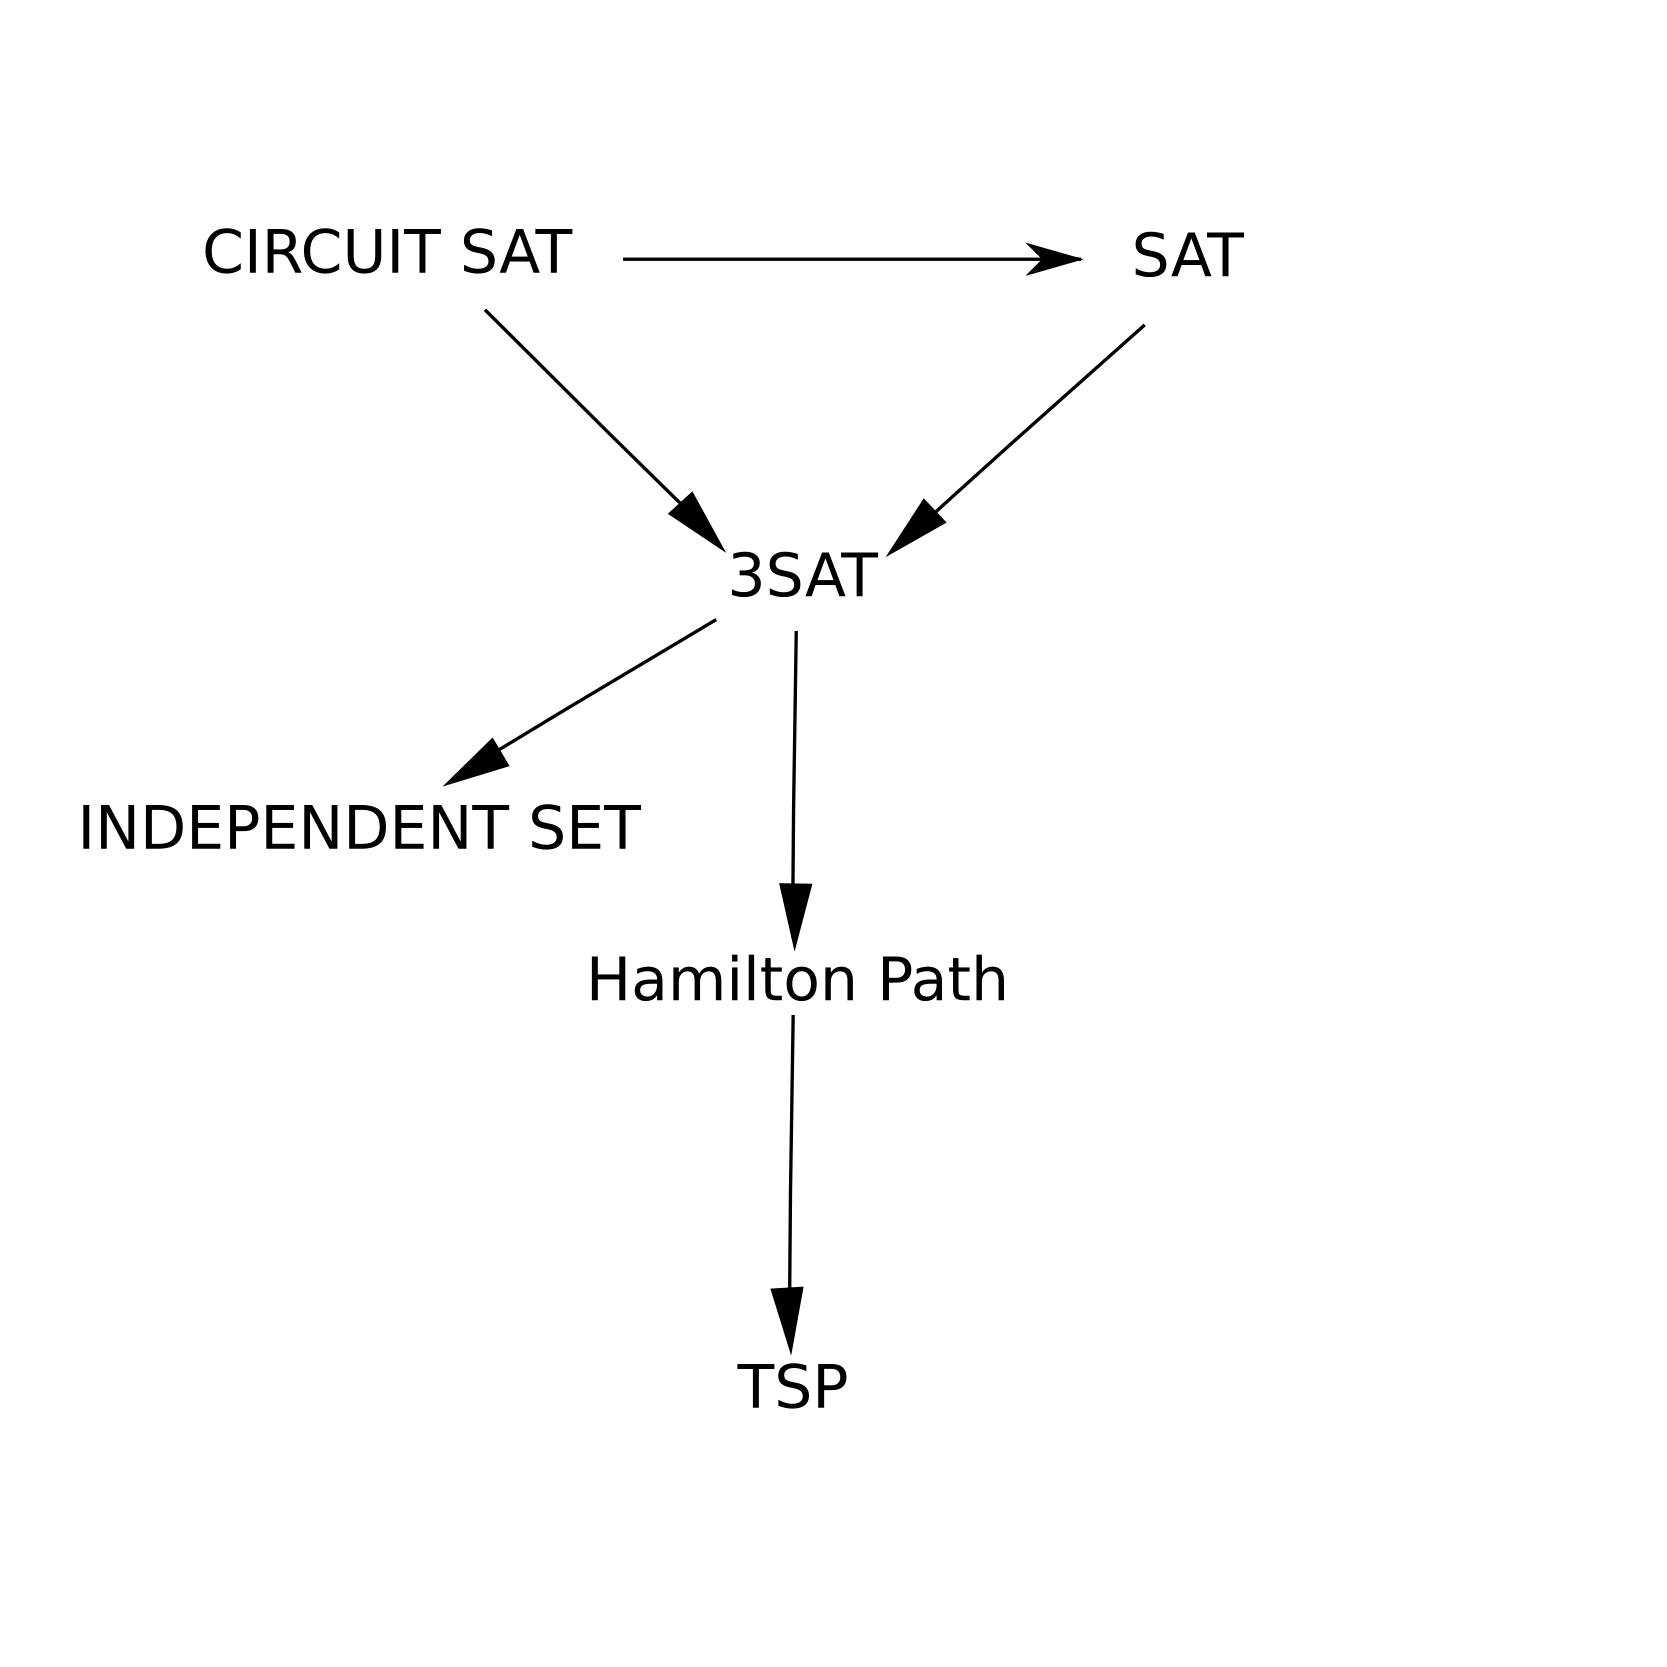
\includegraphics[bb=0 0 400 400,scale=0.5]{./GraphReductionTree.png}
 % GraphReductionTree.png: 1667x1667 pixel, 300dpi, 14.11x14.11 cm, bb=0 0 400 400
\end{center}

Vi vil derfor tage et simpelt eksempel først ved at reducere til en special
case af SAT, kaldet 3SAT.\\

3SAT er en special case af SAT hvor hver klausul skal indeholde præcis 3
literals. Det er et specifikt eksempel på kSAT hvor $k \geq 1$.\\
~\\
\textbf{Proposition 9.2:} 3SAT $\in$ NPC

\begin{proof}
 Vi vil, som sagt, vise at 3SAT $\in$ NPC ved at lave en reduktion fra SAT,
 således vi bruger et polynomial time computable map til at oversætte enhver
 instans af SAT til en instans af 3SAT. 

Givet en CNF formel $f$ i SAT vil vi konstrukere en ny CNF formel $f' = r(x)$ i
3SAT med 3 literals i hver klausul. $r$ er således vores polynomial time
computable map der ændrer følgende i $f$:\\

For hver klausul $k$ i $f$ med literals $x_1, \hdots, x_{|k|}$ ændres:
\begin{itemize}
 \item Hvis $|k| = 2$: Dupliker klausulen og tilføj en ny variabel i begge hvor
	 den negeres i anden klausul \\
      $(x_1 \vee x_2) \rightarrow (x_1 \vee x_2 \vee u) \wedge (x_1 \vee x_2 \vee \neg u)$
 \item Hvis $|k| = 1$: Gør som ved $|k| = 2$, men gør det to gange \\
	  $(x_1) \rightarrow (x_1 \vee u_1) \wedge (x_1 \vee \neg u_1) \rightarrow
	  (x_1 \vee u_1 \vee u_2) \wedge (x_1 \vee u_1 \vee \neg u_2) \wedge (x_1
	  \vee \neg u_1 \vee u_2) \wedge (x_1 \vee \neg u_1 \vee \neg u_2)$
 \item Hvis $|k| = 3$: Gør vi ingenting
 \item Hvis $|k| > 3$: Da vi har en klausul $(x_1,\hdots,x_{|k|})$ så skal vi
	 have en generel måde hvorpå vi kan konvertere dette til klausuler med 3
	 literals. Måden vi gør det på er ved at lave nye variabler
	 $u_1,\hdots,u_{|k|-3}$ og lave en ``kaskade'' af disse:\\
	  $(x_1,\hdots,x_{|k|}) \rightarrow (x_1 \vee x_2 \vee u_1) \wedge (x_3
	  \vee \neg u_1 \vee u_2) \wedge \hdots \wedge (x_{k-2} \vee \neg u_{k-4}
	  \vee u_{k-3}) \wedge (x_{k-1} \vee x_k \vee \neg u_{k-3})$ \\
      ~\\
      Længden af denne udvidelse er så $|k|-2$.
	  For at se at vi kan gøre dette, så skal vi kigge på hvorledes det gamle
	  udtryk har set ud. Hvis det gamle udtryk har været sandt så har et af
	  $x_i$'erne været sat til true. Hvis vi så sætter alle $u_i$'er til true
	  op til punktet hvor $x_i$ blev mødt og falsk derefter, så kan vi se, at
	  det giver et samlet sandt udtryk som før. Det betyder også at hvis ingen
	  $x_i$'er er sat til true og det samlede udtryk derfor burde være falsk,
	  så har vi også bibeholdt dette i oversættelsen, da alle $u_i$'erne derfor
	  må være false.\\
      ~\\
	  \textbf{TODO:} Ovenstående trin for $|k| > 3$ er IKKE rigtig. Jeg har
	  ikke haft tid til at rette det.. Søg på Google og find det rigtige svar.
	  Der findes sider der beskriver beviset.
\end{itemize}

En tilfredsstillende assignment for $f'$ vil altså også være tilfredsstillende
for $f$ og vice-versa. Vi har således lavet en reduktion vha. et polynomial
time computable map $r$, hvor længden af $f'$ maksimalt er $O(|f|^2)$.

Vi har derfor nu vist, at SAT $\leq$ 3SAT, hvorfor vi kan konkludere at 3SAT
$\in$ NPC.
\end{proof}

\subsubsection{Theorem 9.4}

Nu hvor vi så har 3SAT på plads, så kan vi gå videre og kigge på et grafproblem
kaldet INDEPENDENT SET. Vi har en urettet graf $G=(V,E)$. Lad så $I \subseteq
V$, hvor vi kalder $I$ ``independent'' hvis der for alle $i,j \in I$ ikke er en
kant imellem $i$ og $j$. 

INDEPENDENT SET problemet er så: \textit{Givet en urettet graf $G=(V,E)$ og et
mål $K$, er der et independent set $I$ hvor $|I|=K$?}\\
~\\
\textbf{Theorem 9.4:} INDEPENDENT SET $\in$ NPC

\begin{proof}
 For at kunne bevise INDEPENDENT SET er i NPC, så skal vi bruge en lille
 gadget, nemlig en trekant som dem nedenfor. Begrundelsen for dette er, at hvis
 grafen indeholder en trekant, så ved vi på forhånd et independent set
 maksimalt kan indeholde 1 af de 3 knuder i trekanten. Dette bruger vi så i
 beviset ved at vi begrænser den mængde af grafer vi kigger på, til kun at
 tillade grafer vis knuder kan opdeles i $m$ disjunkte trekanter. Således får
 vi at vi maksimalt kan have et independent set af størrelse $m$ (en fra hver
 trekant) og at denne eksisterer hvis og kun hvis kanterne i konstruktionen
 tillader vi kan vælge en knude fra hver trekant.
 \begin{center}
 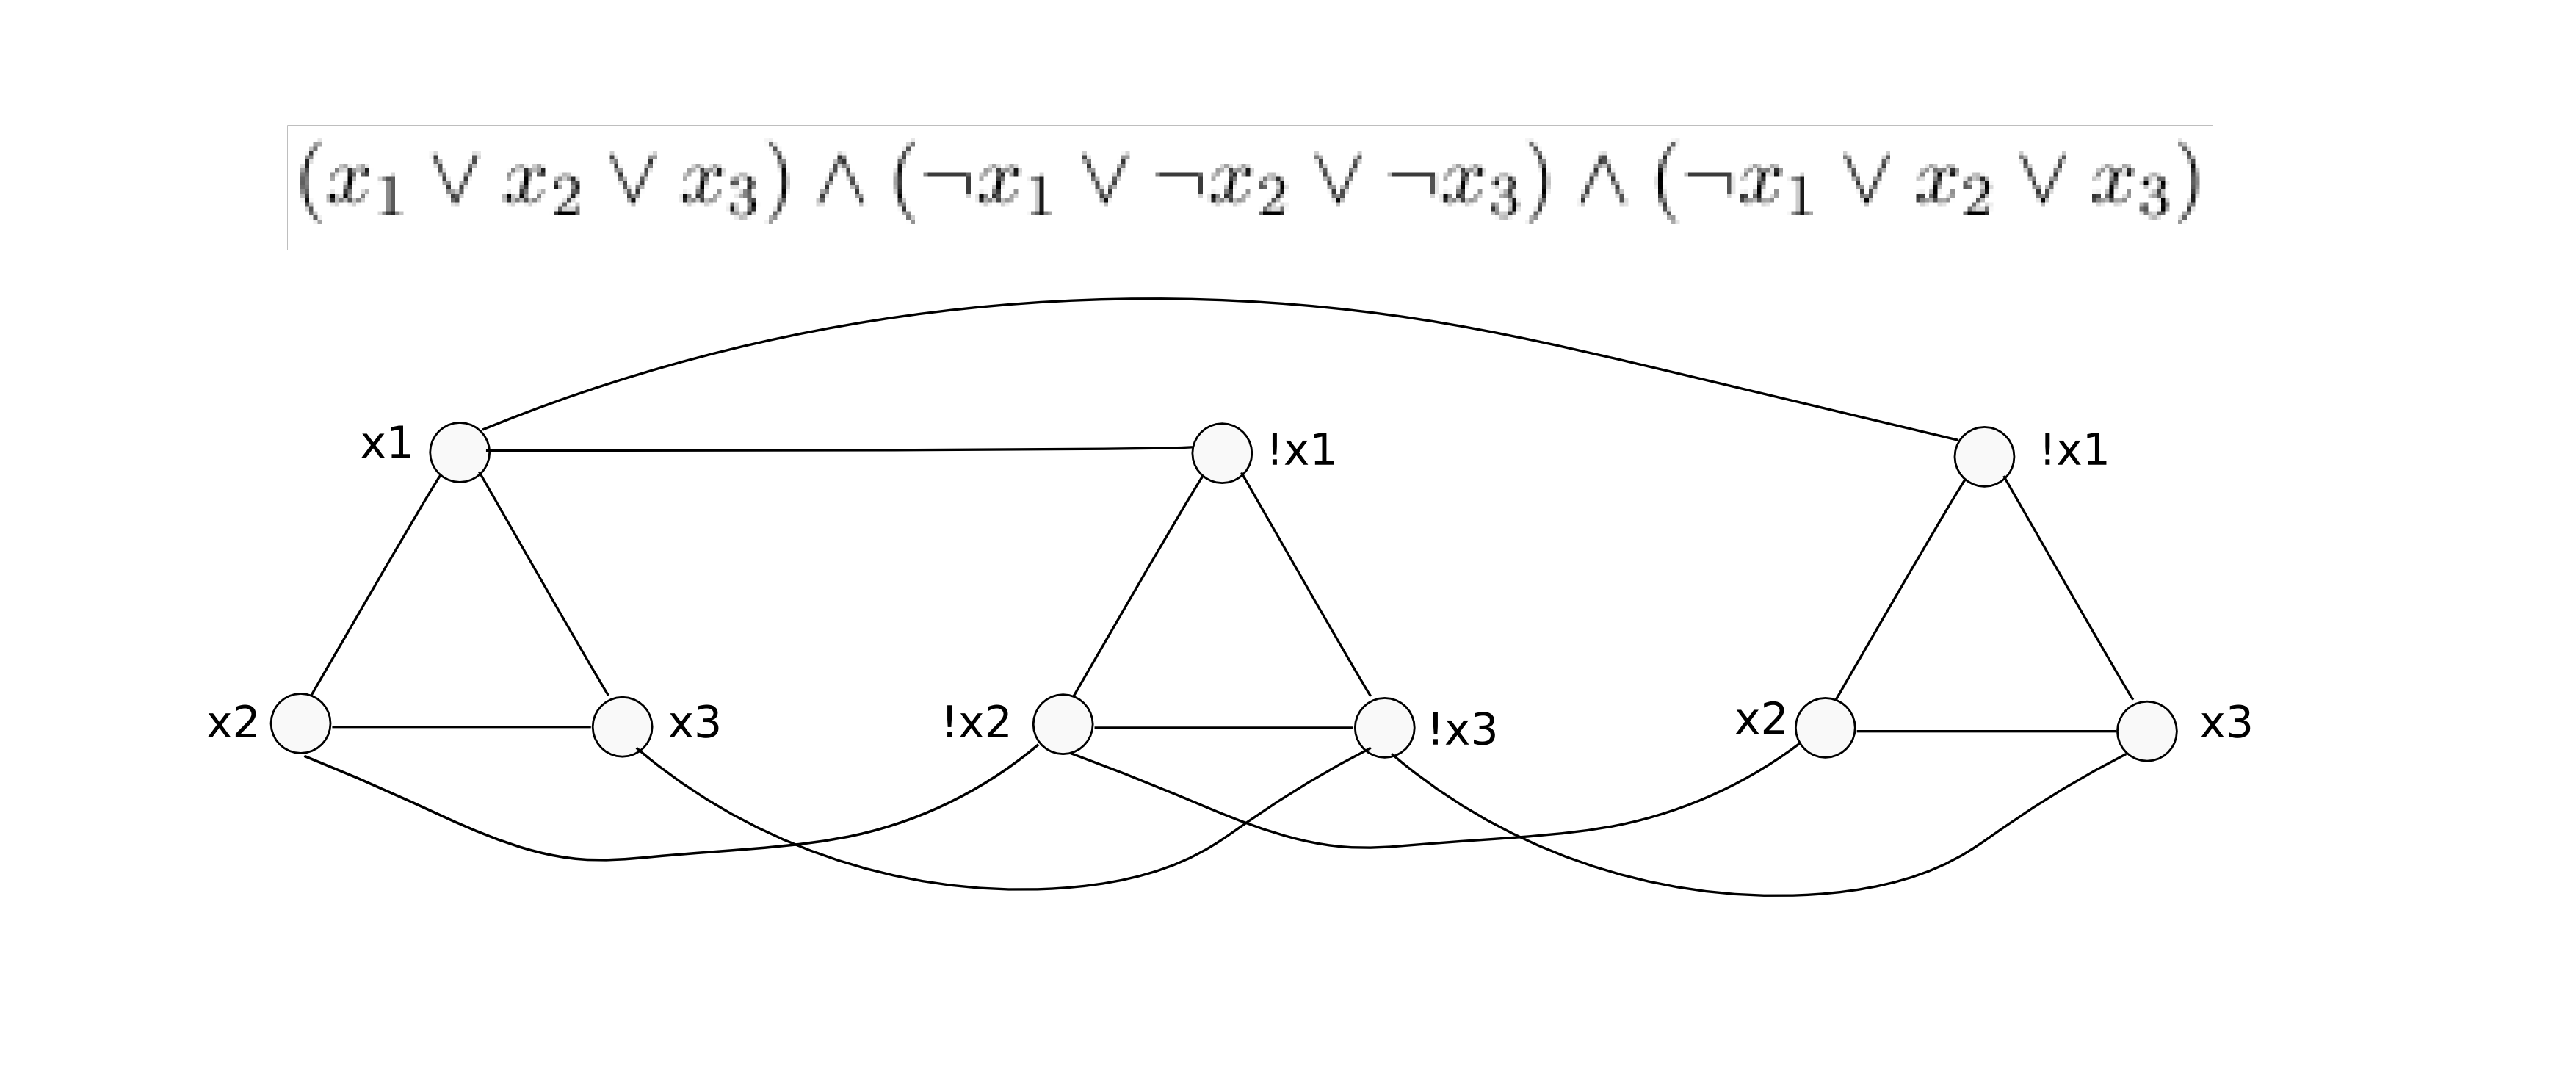
\includegraphics[bb=0 0 842 595,scale=0.5]{./INDEPENDENTSET.png}
 % INDEPENDENTSET.png: 3508x2480 pixel, 300dpi, 29.70x21.00 cm, bb=0 0 842 595
\end{center}
Konstruktionen i reduktionen fra en 3SAT instans til INDEPENDENT SET kommer så
nemt heraf (illustreret ovenfor). Konstruktionen er som følger:

\begin{enumerate}
 \item For hver af de $m$ klausuler af en given CNF formel $f$ skabes en ny
	 trekant i $G$.
 \item Hver knude i trekanten svarer så til en literal i den pågældende klausul.
 \item Tilføj kanter mellem nodes med modsatte literals (således $x_1$ får en
	 kant til $\neg x_1$).
 \item Sæt målet $K$ i INDEPENDENT SET problemet til $m$.
\end{enumerate}

Herefter er konstruktionen færdig. Vi påstår så nu, at der er et independent
set af $K$ nodes i $G$ hvis og kun hvis $f$ tilfredsstilles. Hvis vi antager
sådan et independent set $I$ eksisterer, så siden $K=m$, så må $I$ indeholde en
knude pr. trekant. Siden alle nodes er labeled med deres literal og $I$ ikke
indeholder to knuder svarende til modsatte literals, så er $I$ en sandt/falsk
tildeling der tilfredsstiller $f$. Alle literals indeholdt i $I$ bliver så dem
der er ``true''.

Og set fra den anden side, så hvis vi ved $f$ har en tilfredstillende
tildeling, så identificerer vi blot de literals der bliver ``true'' i $f$ og
markerer dem som en del af $I$ i grafen $G$, hvorved vi får et independent set
med $m=K$ uafhængige knuder.

Vi har derved bevist at 3SAT $\leq$ INDEPENDENT SET, hvorved vi kan konkludere
INDEPENDENT SET $\in$ NPC.
\end{proof}

\subsubsection{Theorem 9.7}

Nu har vi så gået i en retning med reduktioner fra 3SAT og vil nu gå i en ny
retning, nemlig mod problemet HAMILTON PATH. 
HAMILTON PATH problemet er så: \textit{Givet en urettet graf $G=(V,E)$, har $G$
en Hamilton path, altså en sti der besøger hver knude præcis en gang?}\\
~\\
\textbf{Theorem 9.7:} HAMILTON PATH $\in$ NPC

\begin{proof}
 Det vi ønsker at bevise er, at HAMILTON PATH er NP-Complete og måden vi gør
 det på er ved at reducerer fra 3SAT. Så vi skal vise at 3SAT $\leq$ HAMILTON
 PATH.

Så fra 3SAT har vi altså en CNF formel $f$ med variabler $x_1,\hdots,x_n$ og
klausuler $C_1,\hdots,C_m$, hver med 3 literals. Vi konstruerer så en graf $G =
r(f)$ med en Hamilton Path hvis og kun hvis formel $f$ tilfredsstilles.
Vi skal altså finde en måde at modellere 3SAT vha. HAMILTON PATH, således vi
har ækvivalenten af nogle boolske variabler, muligheden for at sætte dem til
sandt/falsk, en ækvivalent af klausuler som constraints, samt muligheden for at
bibeholde konsistens således $x_i$ altid har samme værdi og $\neg x_i$ altid
har den modsatte værdi heraf.\\

I vores tilfælde gør vi dette vha. nogle gadgets. Den første af disse er en
såkaldt ``choice gadget'', som illustreret herunder.
\begin{center}
 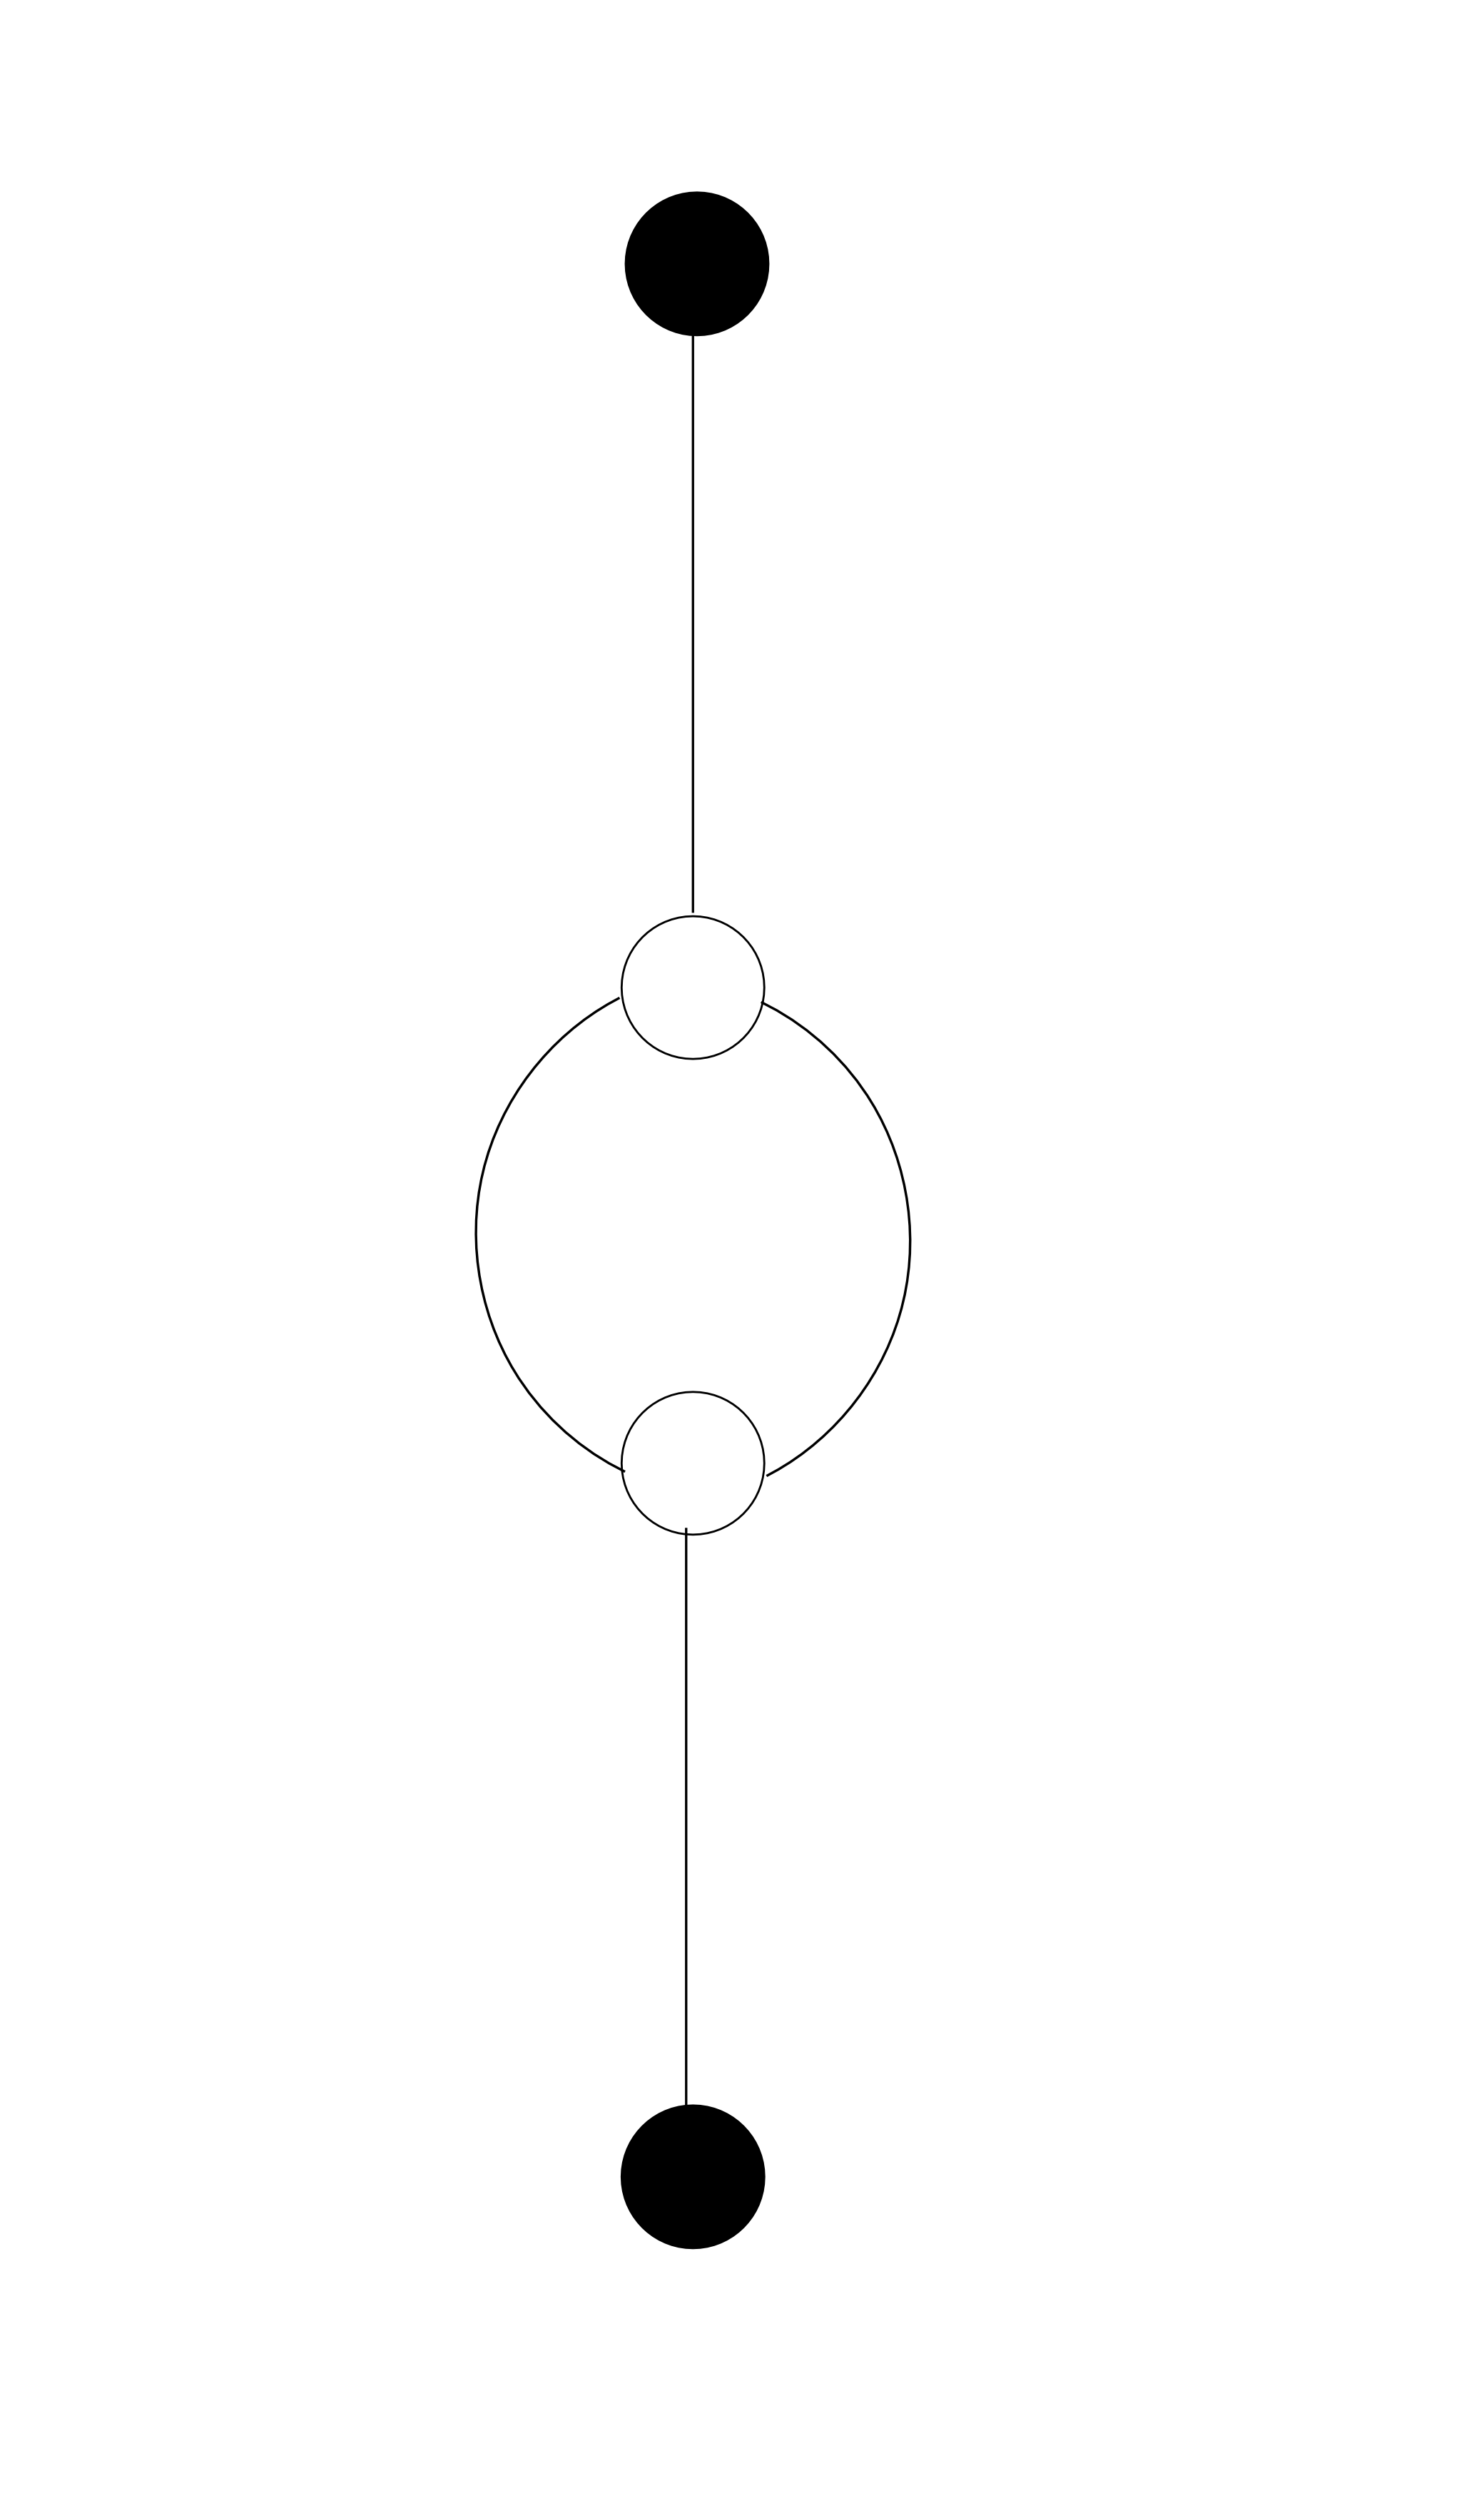
\includegraphics[bb=0 0 499 842,scale=0.2]{./choiceGadget.png}
 % choiceGadget.png: 2080x3508 pixel, 300dpi, 17.61x29.70 cm, bb=0 0 499 842
\end{center}
Denne gadget skal så bruges som en delgraf forbundet til resten vha. de sorte
knuder. Vores choice gadget vil så gøre, at vi kan tildele forskellige
sandhedsværdier afhængig af hvilken kant Hamilton stien vælger ned igennem
delgrafen og derved modellere en boolsk variabel. 

Så nu har vi boolske variabler på plads, nu mangler vi en gadget til at
håndtere consistency. Måden hvorpå vi gør dette er vha. følgende ``consistency
gadget''.

\begin{center}
 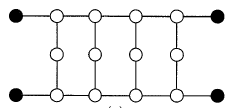
\includegraphics[bb=0 0 173 81]{./consistencyGadget.png}
 % consistencyGadget.: 231x108 pixel, 96dpi, 6.11x2.86 cm, bb=0 0 173 81
\end{center}

Hvis denne gadget kobles til en omkringliggende graf vha. de sorte knuder, så
kan vi se at en given Hamilton Path kun har 2 mulige veje at gå igennem grafen.
Uanset hvad er den nød til at zig-zag op og ned langs grafen for at kunne
besøge alle knuder, så det eneste der kan varieres er hvilken sort knude den
starter udfra. Vi får altså egenskaben, at denne gadget nærmest opfører sig som
to separate kanter hvor en kant besøges af Hamilton stien og den anden gør
ikke. Vi kan altså tænke på denne gadget som en form for XOR mellem to kanter:

\begin{center}
 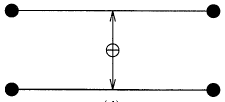
\includegraphics[bb=0 0 173 81]{./consistencyGadget2.png}
 % consistencyGadget.: 231x108 pixel, 96dpi, 6.11x2.86 cm, bb=0 0 173 81
\end{center}

Så nu har vi en consistency gadget på plads, så mangler vi bare at håndtere
klausuler. Men til dette kan vi heldigvis bruge en gammel kending, nemlig
trekanten. Modsat brugen i INDEPENDENT SET, så vælger vi dog her at tildele en
literal til hver kant. Ved at gøre dette, så kan vi sige en given literal er
``false'' såfremt den indgår i den pågældende Hamilton Path. Derved har vi
også, at minimum en literal er nød til at være ``true'', da der ellers ikke er
nogen Hamilton Path. Vores ``constraint gadget'' ser så således ud:

\begin{center}
 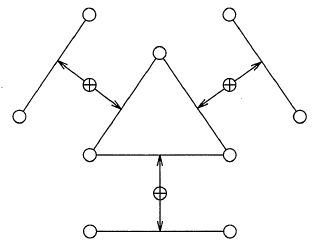
\includegraphics[bb=0 0 241 185]{./constraintGadget.png}
 % constraintGadget.png: 322x247 pixel, 96dpi, 8.52x6.53 cm, bb=0 0 241 185
\end{center}

Hvis vi så sætter alle de her ting sammen så får vi følgende opskrift:\\
\begin{enumerate}
 \item Konstruer en graf $G$ med en start knude kaldet 1.

 \item Lav $n$ kopier af vores ``choice gadget'', en for hver variabel, og
	 forbind dem i en serie efter 1.

 \item Lav $m$ trekanter, en for hver klausul, og forbind dem således kanten
	 der svarer til $x_i$ er forbundet vha. vores ``consistency gadget'' til
	 kanten i vores ``choice gadgets'' der svarer til true-kanten for variablen
	 $x_i$, således trekantens kant traverseres hvis ``choice gadget`` kanten
	 ikke gør. Og tilsvarende hvis en kant svarer til $\neg x_i$ så forbind den
	 vha. en ``consistency gadget'' til false-kanten på den tilsvarende
	 variables ``choice gadget''. 
	 \textit{OBS: der kan godt være flere ``consistency gadgets'' der går til
	 samme kant i en ``choice gadget'', men ikke den anden vej rundt.}

 \item Herefter skabes en clique indeholdende de $3m$ trekant knuder, den
	 sidste knude i serien af ``choice gadgets'', samt en ny knude kaldet 3.
	 \textit{OBS: En clique er bare et sæt af knuder hvor alle mulige kanter
	 eksisterer imellem dem}

 \item Slutteligt tilføjes en enkelt knude kaldet 2 og forbindes til 3.

\end{enumerate}
Herefter har vi konstrueret vores graf, som er illustereret nedenfor:

\begin{center}
 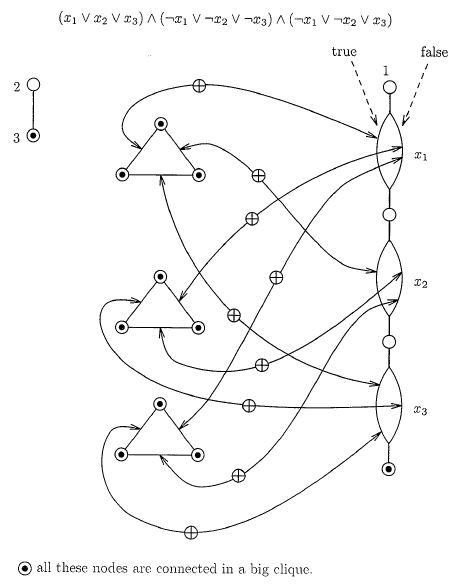
\includegraphics[bb=0 0 350 440]{./hamiltonPath.png}
 % hamiltonPath.png: 467x587 pixel, 96dpi, 12.35x15.53 cm, bb=0 0 350 440
\end{center}

Vi påstår så nu, at grafen har en Hamilton Path hvis og kun hvis $f$ har en
tilfredsstillende tildeling. Lad os antage en sådan Hamilton Path eksisterer,
så må start og slut på stien være henholdsvis knude 1 og knude 2. Hvis vi så
starter fra knude 1, så må stien gå ned igennem de pågældende ``choice
gadgets'' ved enten at tage kanten der svarer til ``true`` eller kanten der
svarer til ''false``. Desuden skal alle XORs traverseres, således vi i sidste
ende får at hele kæden af valg bliver traverseret. Hele denne sti definerer så
en tildeling af sandhedsværdier, som vi kalder $T$. Efter dette traverseres
trekanterne i en eller anden rækkefølge hvorefter vi ender ved knude 2.\\

Vi påstår så $T$ tilfredsstiller $f$, da alle XORs bliver traverseret på en
måde hvor de fungerer som XOR, da en trekants side svarende til en literal, kun
traverseres hvis den literal var ''false``. Derved siden der ingen klausuler er
for hvilket alle literals er ''false``, så er $f$ tilfredsstillet.

Og set fra den anden side hvor vi har en given tildeling $T$ der
tilfredsstiller $f$, så kan vi bruge $r(f)$ til at skabe en graf med en
Hamilton Path der starter fra knude 1. Herefter traverserer den ned igennem
valgmulighederne og følger kanterne svarende til værdierne i $T$. Efter dette
er gjort er resten af grafen en stor clique, som så bliver traverseret indtil
stien slutter ved knude 2.

Vi har således vist at 3SAT $\leq$ HAMILTON PATH, og derved at HAMILTON PATH
$\in$ NPC.
\end{proof}


\subsubsection{Collary: (TSP $\in$ NPC)}

Nu hvor vi har HAMILTON PATH på plads som NPC, så kan vi også slutteligt lige
argumentere for at TSP ligeledes er det, ved at lave et  simpelt bevis.\\

\textbf{Collary: $TSP(D) \in NPC$}

\begin{proof}
 Vi vil vise TSP er NP-Complete ved at reducere fra HAMILTON PATH. Dette gør vi
 ved at vi har en graf $G=(V,E)$ i HAMILTON PATH, og vi vil så konstruere en ny
 graf i TSP således $G' = r(G)$. Hertil skal vi også opbygge en distance matrix
 $d_{ij}$ således følgende gælder:

\begin{itemize}
 \item Hvis $[i,j]$ er en kant i $G$, så sæt $d_{ij}=1$.
 \item Ellers sæt $d_{ij}=2$.
\end{itemize}

Vi skal også have et budget $B$ således at der er en rute af længde $B$ eller
mindre hvis og kun hvis $G$ har en Hamilton Path. Der er desuden $n$ byer, en
for hver knude i grafen $G$. Sidst men ikke mindst sættes $B=n+1$.
Konstruktionen er herefter fuldendt.\\

Vi påstår så nu, at $G'$ har en rute med distance højst $B$ hvis og kun hvis
$G$ har en Hamilton Path. Hvis vi først antager, at $G$ har en Hamilton Path,
så vil der være en rute i $G'$ for hvilken den samlede distance er mindre end
$B$ da $B=n+1$ og der kun er $n$ byer. Hvorimod hvis vi antager der ikke er en
Hamilton Path, så vil der heller ikke være en rute i $G'$ da en given rute vil
have distance på $2(n-1) > B$.

Vi har derved vist at ovenstående er en korrekt reducering af HAMILTON PATH til
TSP, så HAMILTON PATH $\leq$ TSP, og derved gælder der at TSP $\in$ NPC.
\end{proof}
